\documentclass[12pt,]{article}
\usepackage{lmodern}
\usepackage{amssymb,amsmath}
\usepackage{ifxetex,ifluatex}
\usepackage{fixltx2e} % provides \textsubscript
\ifnum 0\ifxetex 1\fi\ifluatex 1\fi=0 % if pdftex
  \usepackage[T1]{fontenc}
  \usepackage[utf8]{inputenc}
\else % if luatex or xelatex
  \ifxetex
    \usepackage{mathspec}
  \else
    \usepackage{fontspec}
  \fi
  \defaultfontfeatures{Ligatures=TeX,Scale=MatchLowercase}
\fi
% use upquote if available, for straight quotes in verbatim environments
\IfFileExists{upquote.sty}{\usepackage{upquote}}{}
% use microtype if available
\IfFileExists{microtype.sty}{%
\usepackage{microtype}
\UseMicrotypeSet[protrusion]{basicmath} % disable protrusion for tt fonts
}{}
\usepackage[margin=1in]{geometry}
\usepackage{hyperref}
\hypersetup{unicode=true,
            pdftitle={STAT 6910: HW 6},
            pdfauthor={David Angeles},
            pdfborder={0 0 0},
            breaklinks=true}
\urlstyle{same}  % don't use monospace font for urls
\usepackage{color}
\usepackage{fancyvrb}
\newcommand{\VerbBar}{|}
\newcommand{\VERB}{\Verb[commandchars=\\\{\}]}
\DefineVerbatimEnvironment{Highlighting}{Verbatim}{commandchars=\\\{\}}
% Add ',fontsize=\small' for more characters per line
\usepackage{framed}
\definecolor{shadecolor}{RGB}{248,248,248}
\newenvironment{Shaded}{\begin{snugshade}}{\end{snugshade}}
\newcommand{\KeywordTok}[1]{\textcolor[rgb]{0.13,0.29,0.53}{\textbf{#1}}}
\newcommand{\DataTypeTok}[1]{\textcolor[rgb]{0.13,0.29,0.53}{#1}}
\newcommand{\DecValTok}[1]{\textcolor[rgb]{0.00,0.00,0.81}{#1}}
\newcommand{\BaseNTok}[1]{\textcolor[rgb]{0.00,0.00,0.81}{#1}}
\newcommand{\FloatTok}[1]{\textcolor[rgb]{0.00,0.00,0.81}{#1}}
\newcommand{\ConstantTok}[1]{\textcolor[rgb]{0.00,0.00,0.00}{#1}}
\newcommand{\CharTok}[1]{\textcolor[rgb]{0.31,0.60,0.02}{#1}}
\newcommand{\SpecialCharTok}[1]{\textcolor[rgb]{0.00,0.00,0.00}{#1}}
\newcommand{\StringTok}[1]{\textcolor[rgb]{0.31,0.60,0.02}{#1}}
\newcommand{\VerbatimStringTok}[1]{\textcolor[rgb]{0.31,0.60,0.02}{#1}}
\newcommand{\SpecialStringTok}[1]{\textcolor[rgb]{0.31,0.60,0.02}{#1}}
\newcommand{\ImportTok}[1]{#1}
\newcommand{\CommentTok}[1]{\textcolor[rgb]{0.56,0.35,0.01}{\textit{#1}}}
\newcommand{\DocumentationTok}[1]{\textcolor[rgb]{0.56,0.35,0.01}{\textbf{\textit{#1}}}}
\newcommand{\AnnotationTok}[1]{\textcolor[rgb]{0.56,0.35,0.01}{\textbf{\textit{#1}}}}
\newcommand{\CommentVarTok}[1]{\textcolor[rgb]{0.56,0.35,0.01}{\textbf{\textit{#1}}}}
\newcommand{\OtherTok}[1]{\textcolor[rgb]{0.56,0.35,0.01}{#1}}
\newcommand{\FunctionTok}[1]{\textcolor[rgb]{0.00,0.00,0.00}{#1}}
\newcommand{\VariableTok}[1]{\textcolor[rgb]{0.00,0.00,0.00}{#1}}
\newcommand{\ControlFlowTok}[1]{\textcolor[rgb]{0.13,0.29,0.53}{\textbf{#1}}}
\newcommand{\OperatorTok}[1]{\textcolor[rgb]{0.81,0.36,0.00}{\textbf{#1}}}
\newcommand{\BuiltInTok}[1]{#1}
\newcommand{\ExtensionTok}[1]{#1}
\newcommand{\PreprocessorTok}[1]{\textcolor[rgb]{0.56,0.35,0.01}{\textit{#1}}}
\newcommand{\AttributeTok}[1]{\textcolor[rgb]{0.77,0.63,0.00}{#1}}
\newcommand{\RegionMarkerTok}[1]{#1}
\newcommand{\InformationTok}[1]{\textcolor[rgb]{0.56,0.35,0.01}{\textbf{\textit{#1}}}}
\newcommand{\WarningTok}[1]{\textcolor[rgb]{0.56,0.35,0.01}{\textbf{\textit{#1}}}}
\newcommand{\AlertTok}[1]{\textcolor[rgb]{0.94,0.16,0.16}{#1}}
\newcommand{\ErrorTok}[1]{\textcolor[rgb]{0.64,0.00,0.00}{\textbf{#1}}}
\newcommand{\NormalTok}[1]{#1}
\usepackage{graphicx,grffile}
\makeatletter
\def\maxwidth{\ifdim\Gin@nat@width>\linewidth\linewidth\else\Gin@nat@width\fi}
\def\maxheight{\ifdim\Gin@nat@height>\textheight\textheight\else\Gin@nat@height\fi}
\makeatother
% Scale images if necessary, so that they will not overflow the page
% margins by default, and it is still possible to overwrite the defaults
% using explicit options in \includegraphics[width, height, ...]{}
\setkeys{Gin}{width=\maxwidth,height=\maxheight,keepaspectratio}
\IfFileExists{parskip.sty}{%
\usepackage{parskip}
}{% else
\setlength{\parindent}{0pt}
\setlength{\parskip}{6pt plus 2pt minus 1pt}
}
\setlength{\emergencystretch}{3em}  % prevent overfull lines
\providecommand{\tightlist}{%
  \setlength{\itemsep}{0pt}\setlength{\parskip}{0pt}}
\setcounter{secnumdepth}{0}
% Redefines (sub)paragraphs to behave more like sections
\ifx\paragraph\undefined\else
\let\oldparagraph\paragraph
\renewcommand{\paragraph}[1]{\oldparagraph{#1}\mbox{}}
\fi
\ifx\subparagraph\undefined\else
\let\oldsubparagraph\subparagraph
\renewcommand{\subparagraph}[1]{\oldsubparagraph{#1}\mbox{}}
\fi

%%% Use protect on footnotes to avoid problems with footnotes in titles
\let\rmarkdownfootnote\footnote%
\def\footnote{\protect\rmarkdownfootnote}

%%% Change title format to be more compact
\usepackage{titling}

% Create subtitle command for use in maketitle
\newcommand{\subtitle}[1]{
  \posttitle{
    \begin{center}\large#1\end{center}
    }
}

\setlength{\droptitle}{-2em}

  \title{STAT 6910: HW 6}
    \pretitle{\vspace{\droptitle}\centering\huge}
  \posttitle{\par}
    \author{David Angeles}
    \preauthor{\centering\large\emph}
  \postauthor{\par}
    \date{}
    \predate{}\postdate{}
  

\begin{document}
\maketitle

\begin{verbatim}
## Warning: package 'emmeans' was built under R version 3.4.4
\end{verbatim}

\begin{verbatim}
## NOTE: As of emmeans versions > 1.2.3,
##       The 'cld' function will be deprecated in favor of 'CLD'.
##       You may use 'cld' only if you have package:multcomp attached.
\end{verbatim}

\subsection{Problem 1}\label{problem-1}

Under what circumstances should the two-way main effects model (6.2.3)
be used rather than the two-way complete model (6.2.2)? {[}1 sentence
may suffice.{]} Discuss the interpretation of main effects in each
model. {[}You can focus on comparing the interpretations of, e.g.,
\(\alpha_1 - \alpha_2\) vs. \(\alpha_1^\star - \alpha_2^\star\) in these
models.{]}

\paragraph{Answer:}\label{answer}

The two-way main effects model (6.2.3) should be used rather than the
two-way complete model (6.2.2) when an experimenter has sufficient
knowledge about the two treatment factors being studied to state with
reasonable certainty that the factors do not interact.

Using the main effects model, one cannot compare the effects of the
different levels of the factors, say level 1 of \(A\), \(\alpha_1\),
with level 2 of \(A\), \(\alpha_2\). Instead, one must compare the
effects of the different levels of \(A\) averaged over the effects of
\(B\). So, \(\alpha_1-\alpha_2\) is not estimable, but
\(\alpha^\star_2-\alpha^\star_1=\bar{\tau}_{2\bullet}-\bar{\tau}_{1\bullet}\)
is estimable.

\subsection{Problem 2}\label{problem-2}

Solution on the very back.

\subsection{Problem 7 part (a)}\label{problem-7-part-a}

The data shown in Table 6.22 are a subset of the data given by Anderson
and McLean (1974) and show the strength of a weld in a steel bar. Two
factors of interest were gage bar setting (the distance the weld die
travels during the automatic weld cycle) and time of welding (total time
of the automatic weld cycle). Assume that the levels of both factors
were selected to be equally spaced.

\begin{Shaded}
\begin{Highlighting}[]
\NormalTok{weld.data =}\StringTok{ }\KeywordTok{read.table}\NormalTok{(}\StringTok{"~/Desktop/Stats 6910/HW_4_and_5/weld.strength.txt"}\NormalTok{, }
                       \DataTypeTok{header =} \OtherTok{TRUE}\NormalTok{)}
\NormalTok{weld.data}\OperatorTok{$}\NormalTok{trtmt <-}\StringTok{ }\KeywordTok{as.factor}\NormalTok{(weld.data}\OperatorTok{$}\NormalTok{trtmt)}
\end{Highlighting}
\end{Shaded}

\begin{enumerate}
\def\labelenumi{(\alph{enumi})}
\tightlist
\item
  Using the cell-means model (6.2.1) for these data, test the hypothesis
  that there is no difference in the effects of the treatment
  combinations on weld strength against the alternative hypothesis that
  at least two treatment combinations have different effects.
\end{enumerate}

\begin{Shaded}
\begin{Highlighting}[]
\NormalTok{cell_model <-}\StringTok{ }\KeywordTok{aov}\NormalTok{(strength }\OperatorTok{~}\StringTok{ }\NormalTok{trtmt , }\DataTypeTok{data =}\NormalTok{ weld.data)}
\end{Highlighting}
\end{Shaded}

\begin{enumerate}
\def\labelenumi{(\alph{enumi})}
\setcounter{enumi}{2}
\tightlist
\item
  Construct an analysis of variance table and test the hypothesis that
  color has no effect in inflation time.
\end{enumerate}

Let \(\tau_{ij}\) be the deviation from the overall mean weld strength,
\(\mu\), when factor \(A\), the gage bar setting, has level \(i\) and
factor \(B\), the time of welding, had level \(j\). Using an
\(\alpha\)-level of \(\alpha = 0.05\), and the following test:

\begin{center}
 The Null Hypothesis of No Effect on Weld Strength  
 $H_0 : \tau_{ij} = 0 \hspace{.2cm }\forall \hspace{.1cm} i=1,2,...,a \text{ and }\forall  \hspace{.1cm} j=1,2,...,b$ \\
 vs. The Alternative Hypothesis of Some Effect on Weld Strength $H_A : \tau_{ij} \neq \tau_{hk}$ for some $i\neq h$ and $j\neq k$ 
\end{center}

\begin{Shaded}
\begin{Highlighting}[]
\KeywordTok{anova}\NormalTok{(cell_model)}
\end{Highlighting}
\end{Shaded}

\begin{verbatim}
## Analysis of Variance Table
## 
## Response: strength
##           Df Sum Sq Mean Sq F value    Pr(>F)    
## trtmt     14 1261.2  90.086  8.2395 0.0001092 ***
## Residuals 15  164.0  10.933                      
## ---
## Signif. codes:  0 '***' 0.001 '**' 0.01 '*' 0.05 '.' 0.1 ' ' 1
\end{verbatim}

From the analysis of variance table we obtain a \(p\)-value equal to
\(0.0001\), which is less that the \(\alpha\)-level of
\(\alpha = 0.05\). Therefore, we can reject the null hypothesis of no
effect on welding strength in favor of the alternative hypothesis of
some effect on welding Strength.

\subsection{Problem 8}\label{problem-8}

For the experiment described in Exercise 7, use the two-way complete
model instead of the equivalent cell means model.

\begin{enumerate}
\def\labelenumi{(\alph{enumi})}
\tightlist
\item
  Test the hypothesis of no interaction between gage bar setting and
  time of weld and state your conclusion.
\end{enumerate}

Let \(\tau_{ij}\) be the deviation from the overall weld strength,
\(\mu\), when factor \(A\), the gage bar setting, has level \(i\) and
factor \(B\), the time of welding, had level \(j\). Using an
\(\alpha\)-level of \(\alpha = 0.05\), since the sample sizes are all
equal, \(r_{ij}=2\), we can use the following test:

\begin{center}
 The Null Hypothesis of No Interaction Between $A$ and $B$  
 $H_0 : (\alpha \beta)_{ij} - (\alpha \beta)_{iq} - (\alpha \beta)_{sj} + (\alpha \beta)_{sq}= 0 \hspace{.2cm }\forall \hspace{.1cm} i<s \text{ and }\forall  \hspace{.1cm} j<j$ \\
 vs. The Alternative Hypothesis of Some Effect on Weld Strength $H_A :  (\alpha \beta)_{ij} - (\alpha \beta)_{iq} \neq (\alpha \beta)_{sj} - (\alpha \beta)_{sq}$ for some $i\neq s$ and $j\neq q$ 
\end{center}

\begin{Shaded}
\begin{Highlighting}[]
\NormalTok{weld.data}\OperatorTok{$}\NormalTok{gage <-}\StringTok{ }\KeywordTok{as.factor}\NormalTok{(weld.data}\OperatorTok{$}\NormalTok{gage)}
\NormalTok{weld.data}\OperatorTok{$}\NormalTok{time <-}\StringTok{ }\KeywordTok{as.factor}\NormalTok{(weld.data}\OperatorTok{$}\NormalTok{time)}
\end{Highlighting}
\end{Shaded}

\begin{Shaded}
\begin{Highlighting}[]
\NormalTok{model_AB <-}\StringTok{ }\KeywordTok{aov}\NormalTok{(strength }\OperatorTok{~}\StringTok{ }\NormalTok{gage}\OperatorTok{*}\NormalTok{time, }\DataTypeTok{data =}\NormalTok{ weld.data)}
\KeywordTok{anova}\NormalTok{(model_AB)}
\end{Highlighting}
\end{Shaded}

\begin{verbatim}
## Analysis of Variance Table
## 
## Response: strength
##           Df Sum Sq Mean Sq F value    Pr(>F)    
## gage       2 278.60 139.300 12.7409 0.0005838 ***
## time       4 385.53  96.383  8.8155 0.0007212 ***
## gage:time  8 597.07  74.633  6.8262 0.0007535 ***
## Residuals 15 164.00  10.933                      
## ---
## Signif. codes:  0 '***' 0.001 '**' 0.01 '*' 0.05 '.' 0.1 ' ' 1
\end{verbatim}

From the analysis of variance table we obtain a \(p\)-value equal to
\(0.0008\), which is less that the \(\alpha\)-level of
\(\alpha = 0.05\). Therefore, we can reject the null hypothesis of no
effect on welding strength in favor of the alternative hypothesis of
some effect on welding strength.

\begin{enumerate}
\def\labelenumi{(\alph{enumi})}
\setcounter{enumi}{1}
\tightlist
\item
  Draw an interaction plot for the two factors Gage bar setting and Time
  of welding. Does your interaction plot support the conclusion of your
  hypothesis test? Explain.
\end{enumerate}

\begin{Shaded}
\begin{Highlighting}[]
\KeywordTok{attach}\NormalTok{(weld.data)}
\KeywordTok{par}\NormalTok{(}\DataTypeTok{mfrow =} \KeywordTok{c}\NormalTok{(}\DecValTok{1}\NormalTok{, }\DecValTok{2}\NormalTok{))}
\KeywordTok{interaction.plot}\NormalTok{(}\DataTypeTok{x.factor =}\NormalTok{ gage, }\DataTypeTok{trace.factor =}\NormalTok{ time, }\DataTypeTok{response =}\NormalTok{ strength,}
\DataTypeTok{col =} \KeywordTok{c}\NormalTok{(}\DecValTok{1}\NormalTok{, }\DecValTok{2}\NormalTok{, }\DecValTok{3}\NormalTok{, }\DecValTok{4}\NormalTok{), }\DataTypeTok{leg.bty =} \StringTok{"o"}\NormalTok{, }\DataTypeTok{leg.bg =} \StringTok{"white"}\NormalTok{) }
\KeywordTok{interaction.plot}\NormalTok{(}\DataTypeTok{x.factor =}\NormalTok{ time, }\DataTypeTok{trace.factor =}\NormalTok{ gage, }\DataTypeTok{response =}\NormalTok{ strength,}
\DataTypeTok{col =} \KeywordTok{c}\NormalTok{(}\DecValTok{1}\NormalTok{, }\DecValTok{2}\NormalTok{, }\DecValTok{3}\NormalTok{), }\DataTypeTok{leg.bty =} \StringTok{"o"}\NormalTok{, }\DataTypeTok{leg.bg =} \StringTok{"white"}\NormalTok{)}
\end{Highlighting}
\end{Shaded}

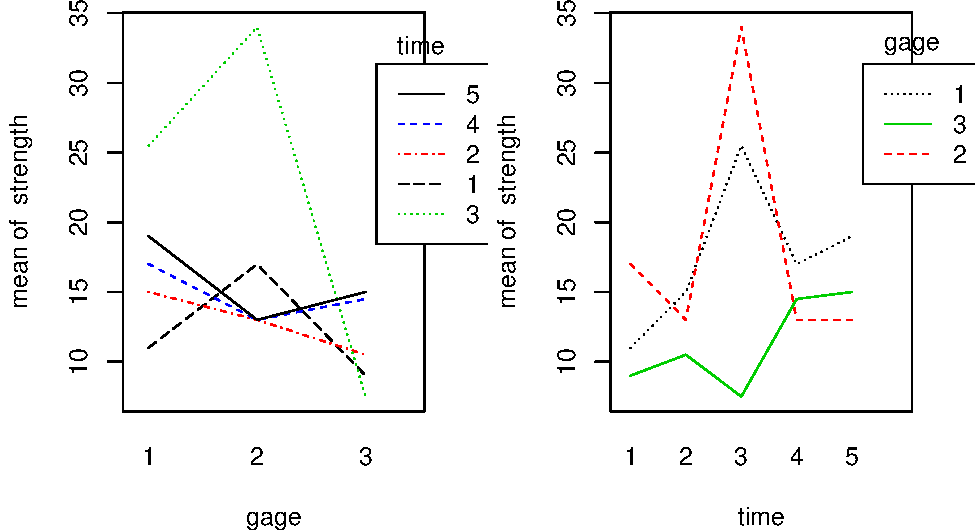
\includegraphics{Markdown_HW_6_files/figure-latex/unnamed-chunk-7-1.pdf}

From the interaction plots above, Mean of Strength vs.~Time, we can see
that the lines aren't parallel and cross multiple times. This implies
that there is definitely some interaction between gage setting and
welding time which supports the conclusion of part (a).

\begin{enumerate}
\def\labelenumi{(\alph{enumi})}
\setcounter{enumi}{2}
\tightlist
\item
  In view of your answer to part (b), is it sensible to investigate the
  differences between the effects of gage bar setting? Why or why not?
  Indicate on your plot what would be compared.
\end{enumerate}

It is not sensible because if we were to compare the differences between
the gage bar settings we would have to compare them averages over
welding time due to the fact that there is some interaction. The
difference between gage bar setting level 2 and level 1 averaged over
welding time is 1.5. However, if we look at the plot, Mean Strength
vs.~Gage, we see that the welding time at level 3 produces a much higher
mean strength when the gage bar setting is at level 2. However, this is
not apparent when we simply observe the difference.

\begin{Shaded}
\begin{Highlighting}[]
\NormalTok{gage_avg <-}\StringTok{ }\KeywordTok{tapply}\NormalTok{(weld.data}\OperatorTok{$}\NormalTok{strength, weld.data}\OperatorTok{$}\NormalTok{gage , mean); gage_avg}
\end{Highlighting}
\end{Shaded}

\begin{verbatim}
##    1    2    3 
## 17.5 18.0 11.3
\end{verbatim}

\subsection{Problem 21}\label{problem-21}

The experiment was run in order to examine the amount of time taken to
boil a given amount of water on the four different burners of her stove,
and with 0, 2, 4, or 6 teaspoons of salt added to the water. Thus the
experiment had two treatment factors with four levels each. The
experimenter ran the experiment as a completely randomized design by
taking \(r = 3\) observations on each of the 16 treatment combinations
in a random order. The data are shown in Table 6.26. The experimenter
believed that there would be no interaction between the two factors.

\begin{Shaded}
\begin{Highlighting}[]
\NormalTok{boiling.data =}\StringTok{ }\KeywordTok{read.table}\NormalTok{(}\StringTok{"~/Desktop/Stats 6910/HW_4_and_5/water.boiling.txt"}\NormalTok{, }
                            \DataTypeTok{header =} \OtherTok{TRUE}\NormalTok{)}
\CommentTok{# make salt and burner factors and add column of two digit treatment combination}
\NormalTok{boiling.data <-}\StringTok{ }\KeywordTok{within}\NormalTok{(boiling.data,\{}
\NormalTok{   f_salt =}\StringTok{ }\KeywordTok{factor}\NormalTok{(salt); f_burner =}\StringTok{ }\KeywordTok{factor}\NormalTok{(burner)}
\NormalTok{   trtmt=}\StringTok{ }\KeywordTok{factor}\NormalTok{(}\DecValTok{10}\OperatorTok{*}\NormalTok{burner }\OperatorTok{+}\StringTok{ }\NormalTok{salt)\})}
\CommentTok{# Display boiling.data}
\KeywordTok{head}\NormalTok{(boiling.data, }\DecValTok{10}\NormalTok{)}
\end{Highlighting}
\end{Shaded}

\begin{verbatim}
##    salt burner time order trtmt f_burner f_salt
## 1     0      1    7     7    10        1      0
## 2     0      1    8    21    10        1      0
## 3     0      1    7    30    10        1      0
## 4     0      2    4     6    20        2      0
## 5     0      2    4    20    20        2      0
## 6     0      2    4    27    20        2      0
## 7     0      3    6     9    30        3      0
## 8     0      3    7    16    30        3      0
## 9     0      3    6    22    30        3      0
## 10    0      4    9    29    40        4      0
\end{verbatim}

\begin{enumerate}
\def\labelenumi{(\alph{enumi})}
\tightlist
\item
  Check the assumptions on the two-way main-effects model.
\end{enumerate}

\begin{Shaded}
\begin{Highlighting}[]
\NormalTok{two.way_model <-}\StringTok{ }\KeywordTok{aov}\NormalTok{(time }\OperatorTok{~}\StringTok{ }\NormalTok{f_salt}\OperatorTok{+}\NormalTok{f_burner, }\DataTypeTok{data =}\NormalTok{ boiling.data)}

\NormalTok{boiling.data =}\StringTok{ }\KeywordTok{within}\NormalTok{(boiling.data, \{}
  \CommentTok{# Compute predicted, residual, and standardized residual values}
\NormalTok{  ypred =}\StringTok{ }\KeywordTok{fitted}\NormalTok{(two.way_model)}
\NormalTok{  e =}\StringTok{ }\KeywordTok{resid}\NormalTok{(two.way_model) }
\NormalTok{  z =}\StringTok{ }\KeywordTok{rstandard}\NormalTok{(two.way_model)\})}
\CommentTok{# Display first 10 lines of boiling.data, 4 digits per variable}
\KeywordTok{print}\NormalTok{(}\KeywordTok{head}\NormalTok{(boiling.data, }\DecValTok{10}\NormalTok{), }\DataTypeTok{digits =} \DecValTok{4}\NormalTok{)}
\end{Highlighting}
\end{Shaded}

\begin{verbatim}
##    salt burner time order trtmt f_burner f_salt          z          e
## 1     0      1    7     7    10        1      0  2.502e-14  1.588e-14
## 2     0      1    8    21    10        1      0  1.576e+00  1.000e+00
## 3     0      1    7    30    10        1      0  0.000e+00 -3.965e-15
## 4     0      2    4     6    20        2      0 -7.878e-01 -5.000e-01
## 5     0      2    4    20    20        2      0 -7.878e-01 -5.000e-01
## 6     0      2    4    27    20        2      0 -7.878e-01 -5.000e-01
## 7     0      3    6     9    30        3      0 -6.565e-01 -4.167e-01
## 8     0      3    7    16    30        3      0  9.191e-01  5.833e-01
## 9     0      3    6    22    30        3      0 -6.565e-01 -4.167e-01
## 10    0      4    9    29    40        4      0  3.939e-01  2.500e-01
##    ypred
## 1  7.000
## 2  7.000
## 3  7.000
## 4  4.500
## 5  4.500
## 6  4.500
## 7  6.417
## 8  6.417
## 9  6.417
## 10 8.750
\end{verbatim}

\begin{Shaded}
\begin{Highlighting}[]
\CommentTok{# Generate residual plots }
\KeywordTok{par}\NormalTok{(}\DataTypeTok{mfrow =} \KeywordTok{c}\NormalTok{(}\DecValTok{1}\NormalTok{,}\DecValTok{3}\NormalTok{))}
\KeywordTok{plot}\NormalTok{(z }\OperatorTok{~}\StringTok{ }\NormalTok{order, }\DataTypeTok{data=}\NormalTok{boiling.data, }
     \DataTypeTok{main=} \StringTok{"Order vs. Std. Residuals"}\NormalTok{,}
     \DataTypeTok{ylab=}\StringTok{"Std. Residuals"}\NormalTok{, }\DataTypeTok{las=}\DecValTok{1}\NormalTok{)}
\KeywordTok{abline}\NormalTok{(}\DataTypeTok{h=}\DecValTok{0}\NormalTok{)}
\KeywordTok{plot}\NormalTok{(z }\OperatorTok{~}\StringTok{ }\NormalTok{ypred, }\DataTypeTok{data=}\NormalTok{boiling.data, }
      \DataTypeTok{main=} \StringTok{"Fitted Values vs. Std. Residuals"}\NormalTok{,}
     \DataTypeTok{ylab=}\StringTok{"Std. Residuals"}\NormalTok{, }\DataTypeTok{las=}\DecValTok{1}\NormalTok{)}
\KeywordTok{abline}\NormalTok{(}\DataTypeTok{h=}\DecValTok{0}\NormalTok{)}
\KeywordTok{qqnorm}\NormalTok{(boiling.data}\OperatorTok{$}\NormalTok{z)}
\CommentTok{# Line through 1st and 3rd quantile points}
\KeywordTok{qqline}\NormalTok{(boiling.data}\OperatorTok{$}\NormalTok{z) }
\end{Highlighting}
\end{Shaded}

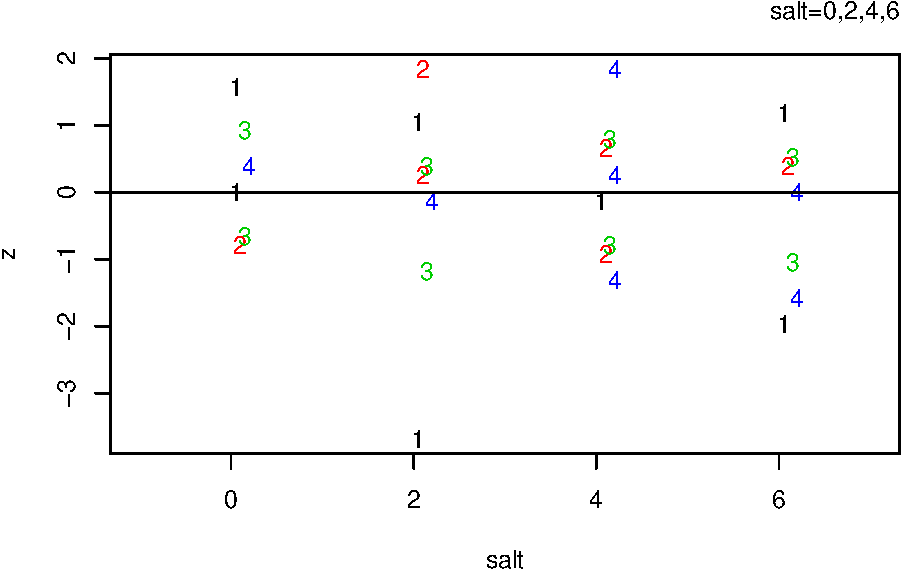
\includegraphics{Markdown_HW_6_files/figure-latex/unnamed-chunk-10-1.pdf}

Assumption (a): The error have mean 0:

\begin{Shaded}
\begin{Highlighting}[]
\KeywordTok{attach}\NormalTok{(boiling.data)}
\end{Highlighting}
\end{Shaded}

\begin{verbatim}
## The following objects are masked from weld.data:
## 
##     time, trtmt
\end{verbatim}

\begin{Shaded}
\begin{Highlighting}[]
\KeywordTok{plot}\NormalTok{(z }\OperatorTok{~}\StringTok{ }\NormalTok{salt, }\DataTypeTok{xaxt =} \StringTok{"n"}\NormalTok{, }\DataTypeTok{type =} \StringTok{"n"}\NormalTok{, }\DataTypeTok{xlim =} \KeywordTok{c}\NormalTok{(}\OperatorTok{-}\DecValTok{1}\NormalTok{, }\DecValTok{7}\NormalTok{)) }\CommentTok{# Suppress x-axis, pts}
\KeywordTok{axis}\NormalTok{(}\DecValTok{1}\NormalTok{, }\DataTypeTok{at =} \KeywordTok{c}\NormalTok{(}\DecValTok{0}\NormalTok{, }\DecValTok{2}\NormalTok{, }\DecValTok{4}\NormalTok{,}\DecValTok{6}\NormalTok{))}
\KeywordTok{points}\NormalTok{(}\DataTypeTok{x =} \KeywordTok{as.numeric}\NormalTok{(salt) }\OperatorTok{+}\StringTok{ }\KeywordTok{as.numeric}\NormalTok{(burner) }\OperatorTok{*}\StringTok{ }\FloatTok{0.05}\NormalTok{, }\DataTypeTok{y =}\NormalTok{ z,}
\DataTypeTok{pch =} \KeywordTok{as.character}\NormalTok{(}\KeywordTok{as.numeric}\NormalTok{(burner)), }\DataTypeTok{col =} \KeywordTok{as.numeric}\NormalTok{(burner)) }
\KeywordTok{mtext}\NormalTok{(}\StringTok{"salt=0,2,4,6"}\NormalTok{, }\DataTypeTok{side =} \DecValTok{3}\NormalTok{, }\DataTypeTok{adj =} \DecValTok{1}\NormalTok{, }\DataTypeTok{line =} \DecValTok{1}\NormalTok{)}
\KeywordTok{abline}\NormalTok{(}\DataTypeTok{h =} \DecValTok{0}\NormalTok{) }\CommentTok{# Horizontal line at zero}
\end{Highlighting}
\end{Shaded}

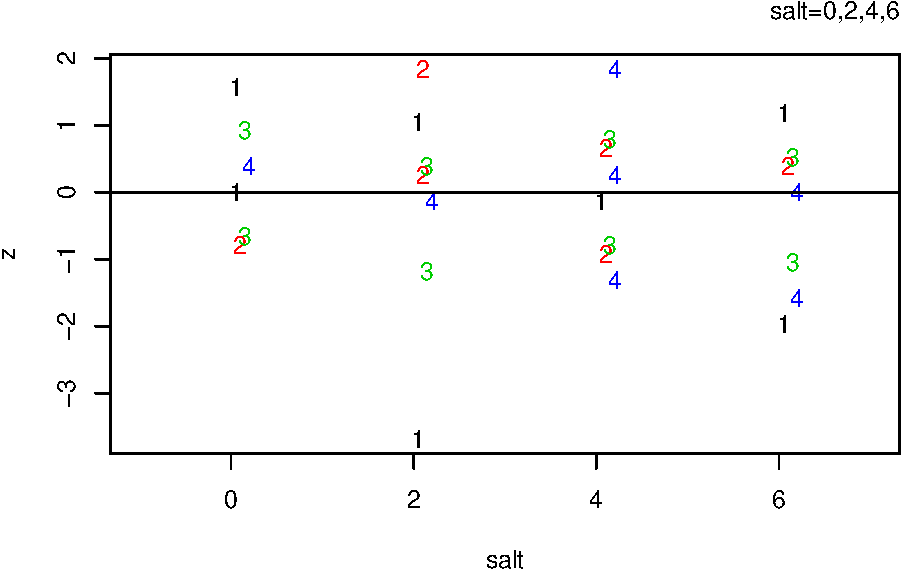
\includegraphics{Markdown_HW_6_files/figure-latex/unnamed-chunk-11-1.pdf}

\begin{Shaded}
\begin{Highlighting}[]
 \CommentTok{# Margin text, top-rt, line 1 abline(h = 0)}
\end{Highlighting}
\end{Shaded}

From the plot above we can see that the burner factor with level 2 is
consistently above or below the 0 line, except for when the salt level
is 4, which is an indication that the the errors do not have mean zero
and therefore the two-way main effects model is probably not the best
model to represent the data.

Assumption (b): The error have constant variance:

\begin{Shaded}
\begin{Highlighting}[]
\NormalTok{Y_i_var <-}\StringTok{ }\KeywordTok{tapply}\NormalTok{(boiling.data}\OperatorTok{$}\NormalTok{z, boiling.data}\OperatorTok{$}\NormalTok{salt, var); Y_i_var}
\end{Highlighting}
\end{Shaded}

\begin{verbatim}
##         0         2         4         6 
## 0.5924765 1.9090909 0.8369906 1.0250784
\end{verbatim}

\begin{Shaded}
\begin{Highlighting}[]
\NormalTok{Y_j_var <-}\StringTok{ }\KeywordTok{tapply}\NormalTok{(boiling.data}\OperatorTok{$}\NormalTok{z, boiling.data}\OperatorTok{$}\NormalTok{burner, var); Y_j_var}
\end{Highlighting}
\end{Shaded}

\begin{verbatim}
##         1         2         3         4 
## 2.2664577 0.7241379 0.6300940 0.7429467
\end{verbatim}

\begin{Shaded}
\begin{Highlighting}[]
\NormalTok{Y_ij_var <-}\StringTok{ }\KeywordTok{tapply}\NormalTok{(boiling.data}\OperatorTok{$}\NormalTok{z, boiling.data}\OperatorTok{$}\NormalTok{trtmt, var); Y_ij_var}
\end{Highlighting}
\end{Shaded}

\begin{verbatim}
##           10           12           14           16           20 
## 8.275862e-01 7.448276e+00 0.000000e+00 3.310345e+00 4.509449e-29 
##           22           24           26           30           32 
## 8.275862e-01 8.275862e-01 0.000000e+00 8.275862e-01 8.275862e-01 
##           34           36           40           42           44 
## 8.275862e-01 8.275862e-01 0.000000e+00 0.000000e+00 2.482759e+00 
##           46 
## 8.275862e-01
\end{verbatim}

\begin{Shaded}
\begin{Highlighting}[]
\KeywordTok{max}\NormalTok{(Y_ij_var)}\OperatorTok{/}\KeywordTok{min}\NormalTok{(Y_ij_var)}
\end{Highlighting}
\end{Shaded}

\begin{verbatim}
## [1] Inf
\end{verbatim}

By plotting the standardized residuals against the fitted values we can
see that the spread of the standardized residuals are roughly centered
around zero. However there seems to be one apparent outlier. Hence, with
these two results we feel comfortable to say that the equal variance
assumption is roughly satisfied.

Assumption (c): The error are normally distributed:

From the qq-plot above we see that the data is fairly straight. However,
there is just one apparent outliers. Therefore, the normality assumption
is reasonable.

Assumption (d): The errors are independent:

From the plot of Order vs.~Std. Residuals we can see that there isn't an
apparent pattern as time increases. Therefore we feel comfortable to say
that the assumption that errors are independent is approximately
satisfies.

\begin{enumerate}
\def\labelenumi{(\alph{enumi})}
\setcounter{enumi}{1}
\tightlist
\item
  Calculate a 99\% set of Tukey confidence intervals for pairwise
  differences between the levels of salt, and calculate separately a
  99\% set of intervals for pairwise differences between the levels of
  burner.
\end{enumerate}

\begin{Shaded}
\begin{Highlighting}[]
\NormalTok{em.salt <-}\StringTok{ }\KeywordTok{emmeans}\NormalTok{(two.way_model, }\DataTypeTok{specs =} \OperatorTok{~}\NormalTok{f_salt)}
\NormalTok{em.burner <-}\StringTok{ }\KeywordTok{emmeans}\NormalTok{(two.way_model, }\DataTypeTok{specs =} \OperatorTok{~}\NormalTok{f_burner)}

\KeywordTok{summary}\NormalTok{(}\KeywordTok{contrast}\NormalTok{(em.salt, }\DataTypeTok{method =} \StringTok{"tukey"}\NormalTok{),}\DataTypeTok{infer =} \KeywordTok{c}\NormalTok{(}\OtherTok{TRUE}\NormalTok{,}\OtherTok{TRUE}\NormalTok{))}
\end{Highlighting}
\end{Shaded}

\begin{verbatim}
##  contrast    estimate        SE df      lower.CL     upper.CL t.ratio
##  0 - 2     0.66666667 0.2803405 41 -0.0839785177 1.4173118510   2.378
##  0 - 4    -0.08333333 0.2803405 41 -0.8339785177 0.6673118510  -0.297
##  0 - 6     0.75000000 0.2803405 41 -0.0006451843 1.5006451843   2.675
##  2 - 4    -0.75000000 0.2803405 41 -1.5006451843 0.0006451843  -2.675
##  2 - 6     0.08333333 0.2803405 41 -0.6673118510 0.8339785177   0.297
##  4 - 6     0.83333333 0.2803405 41  0.0826881490 1.5839785177   2.973
##  p.value
##   0.0974
##   0.9907
##   0.0503
##   0.0503
##   0.9907
##   0.0244
## 
## Results are averaged over the levels of: f_burner 
## Confidence level used: 0.95 
## Conf-level adjustment: tukey method for comparing a family of 4 estimates 
## P value adjustment: tukey method for comparing a family of 4 estimates
\end{verbatim}

From the table above we see that none of the \(p\)-values are below
\(\alpha = .01\), so we cannot detect any pairwise differences between
the salt levels at the \(\alpha=.05\) \(\alpha\)-level. Equivalently,
all the confidence intervals contain zero.

\begin{Shaded}
\begin{Highlighting}[]
\KeywordTok{summary}\NormalTok{(}\KeywordTok{contrast}\NormalTok{(em.burner, }\DataTypeTok{method =}\StringTok{"tukey"}\NormalTok{), }\DataTypeTok{infer =} \KeywordTok{c}\NormalTok{(}\OtherTok{TRUE}\NormalTok{,}\OtherTok{TRUE}\NormalTok{))}
\end{Highlighting}
\end{Shaded}

\begin{verbatim}
##  contrast   estimate        SE df   lower.CL   upper.CL t.ratio p.value
##  1 - 2     2.5000000 0.2803405 41  1.7493548  3.2506452   8.918  <.0001
##  1 - 3     0.5833333 0.2803405 41 -0.1673119  1.3339785   2.081  0.1764
##  1 - 4    -1.7500000 0.2803405 41 -2.5006452 -0.9993548  -6.242  <.0001
##  2 - 3    -1.9166667 0.2803405 41 -2.6673119 -1.1660215  -6.837  <.0001
##  2 - 4    -4.2500000 0.2803405 41 -5.0006452 -3.4993548 -15.160  <.0001
##  3 - 4    -2.3333333 0.2803405 41 -3.0839785 -1.5826881  -8.323  <.0001
## 
## Results are averaged over the levels of: f_salt 
## Confidence level used: 0.95 
## Conf-level adjustment: tukey method for comparing a family of 4 estimates 
## P value adjustment: tukey method for comparing a family of 4 estimates
\end{verbatim}

From the table above we see that only once of the \(p\)-values is not
below \(\alpha = .01\), so we cannot detect any differences between the
burner level 1 and burner level 2 at the \(\alpha=.05\)
\(\alpha\)-level. Equivalently, the confidence interval for
\(\tau_1 - \tau_3\) is the only interval that contain zero.


\end{document}
